\chapter{Related Works}

\section{AI Technology for Generating Pictures}
 The use of AI technology to generate paintings has been heavily researched and has 
made significant progress. This research will enable people who don't have specialized 
skills and knowledge in creating art to generate pictures, as well as provide 
assistance tools for professional artists to use in their creations.
The method using neural networks as a generative tool is typically formulated as a 
pixel-wise mapping \cite{DBLP:journals/corr/JohnsonAL16} or a continuous optimization 
process in pixel space \cite{Gatys_2016_CVPR}. However, it is difficult for neural 
networks to imitate the way humans both create the final image and the process of 
drawing it. Humans typically start by applying rough colors and then gradually adding 
details, while neural networks generate images pixel by pixel. To imitate the human 
drawing process, the machine would have the ability to decompose a given image into 
an ordered sequence of strokes. While neural networks can create sketches \cite{DBLP:journals/corr/HaE17, DBLP:journals/corr/abs-1805-00247}
and doodles \cite{DBLP:journals/corr/abs-1810-05977} with a small number of strokes, 
creating a texture-rich painting requires many more strokes. This makes it difficult 
to set loss functions for each stroke and prepare ground-truth strokes. As a result, 
Reinforcement Learning (RL) is often used to decompose strokes in texture-rich images.
\cite{DBLP:journals/corr/abs-1804-01118, DBLP:journals/corr/abs-1206-4634, Huang_2019_ICCV}
Because the computational cost is high in the learning process of an LR agent, there 
are also studies that have formulated this process as a stroke parameter search. 
\cite{liu2021paint} 
The brush style transfers addressed in this paper are similar to those addressed in
\textit{Neural Style Transfer} \cite{Gatys_2016_CVPR}, in which the overall mood of 
an input style image (such as a painting) is transferred to another image, using CNNs.
That paper is the spark for an approach that utilizes neural networks for Style Transfer. 

Section 3.2 provides an in-depth explanation of \textit{Neural Style Transfer} 
\cite{Gatys_2016_CVPR}.
Section 3.3 covers a method for generating pictures in a human-like process using 
RL \cite{Huang_2019_ICCV}.
Finally, Section 3.4 covers a different approach for generating pictures using FNNs
\cite{liu2021paint}.

\section{Image Style Transfer}
 Gatys \textit{et al}. \cite{Gatys_2016_CVPR} introduced \textit{A Neural Algorithm 
of Artistic Style} which enables the creation of novel images that seamlessly blend 
the subject matter of a photograph with the artistic style of a famous artwork.
In rendering the semantic content of an image in various styles, the problem was
the lack of effective image representations that can explicitly encode semantic 
information and separate image content and style. 
\textit{A Neural Algorithm of Artistic Style} \cite{Gatys_2016_CVPR} is able to 
analyze the visual characteristics of an image and separate them into two distinct 
components: the content and the style.
The content refers to the subject or object depicted in the image, while the style 
refers to the visual techniques manifested in a painting, such as touch and mood.

The algorithm in the paper uses a convolutional neural network (CNN) to extract
content and style features from two input images. The goal is to generate an 
output image that minimizes the difference between the content and style features 
of the input and output images, as measured by two loss functions defined in the 
paper. 

To minimize the difference in content features between the input and output images,
it is necessary to consider reducing the content loss function. 
Let $\vec{p}$ and $\vec{x}$ be the input image and the image that is generated by
the model, and  $P^l$ and $F^l$ be their feature representations of these images in 
layer l of the CNN. Then the loss function of the content of images is defined as:

\begin{equation}
    \label{contentloss}
    \mathcal{ L}_{content}(\vec{p}, \vec{x}, l)=\frac{1}{2} \sum_{i, j}\left(F_{i j}^l-P_{i j}^l\right)^2
\end{equation}
Similarly, to minimize the difference in style features between the input and
output images, we consider reducing the style loss function. The style of an 
image can be represented by the correlations of the outputs of the filters in 
each layer. This feature correlation is given by a Gram matrix, which is 
expressed as:
\begin{equation}
    G_{i j}^l = \sum_k F_{i k}^l F_{j k}^l 
    \label{gram}
\end{equation}
Let $\vec{a}$ and $\vec{x}$ be the input image and the image that is generated by
the model, and $A^l$ and $G^l$ be their style representations of these images in 
layer $l$ of the CNN. The contribution of layer $l$ to the total loss can be 
expressed as:
\begin{equation}
    E_l=\frac{1}{4 N_l^2 M_l^2} \sum_{i, j}\left(G_{i j}^l-A_{i j}^l\right)^2
\end{equation}
Based on this, we can define the loss function for the style of images as:
\begin{equation}
    \label{styleloss}
    \mathcal{ L}_{style}(\vec{a}, \vec{x})=\sum_{l=0}^\mathcal{ L}w_{l}E_{l}
\end{equation}
To transfer the style of image $\vec{a}$ to image $\vec{p}$, it is needed to 
create a new image that maintains the content representation of $\vec{p}$ 
while adopting the style representation of $\vec{a}$. To achieve this, we must 
minimize both Equation \eqref{contentloss} and Equation \eqref{styleloss}.
The final loss function to minimize is:

\begin{equation}
    \mathcal{ L}_{total}(\vec{p}, \vec{a}, \vec{x})=\alpha\mathcal{ L}_{content}(\vec{p}, \vec{x})+\beta\mathcal{ L}_{style}(\vec{a}, \vec{x})
\end{equation}


Figure \ref{output_IST} shows the images generated using this algorithm.
A is the original image, photo from Andreas Praefcke.
In the lower left corner of B through F, the paintings that provided the style 
for each of the generated images are shown.
B : \textit{The Shipwreck of the Minotaur} by J.M.W. Turner, 1805. 
C : \textit{The Starry Night} by Vincent van Gogh, 1889. 
D : \textit{Der Schrei} by Edvard Munch, 1893. 
E : \textit{Femme nue assise} by Pablo Picasso, 1910. 
F : \textit{Composition VII} by Wassily Kandinsky, 1913.

These are high quality paintings to which the style, such as the touch of the 
brush, has been adapted. 
However, the colors of the output picture are those of the style image, 
not the original image, and the result images have the characteristic objects of 
the style image (e.g., the moon, stars, and wavy clouds in \textit{The Starry Night}).
In this paper, we aim to address the problem of transferring only brush style 
in paintings.

\begin{figure}[p]
    \centering
    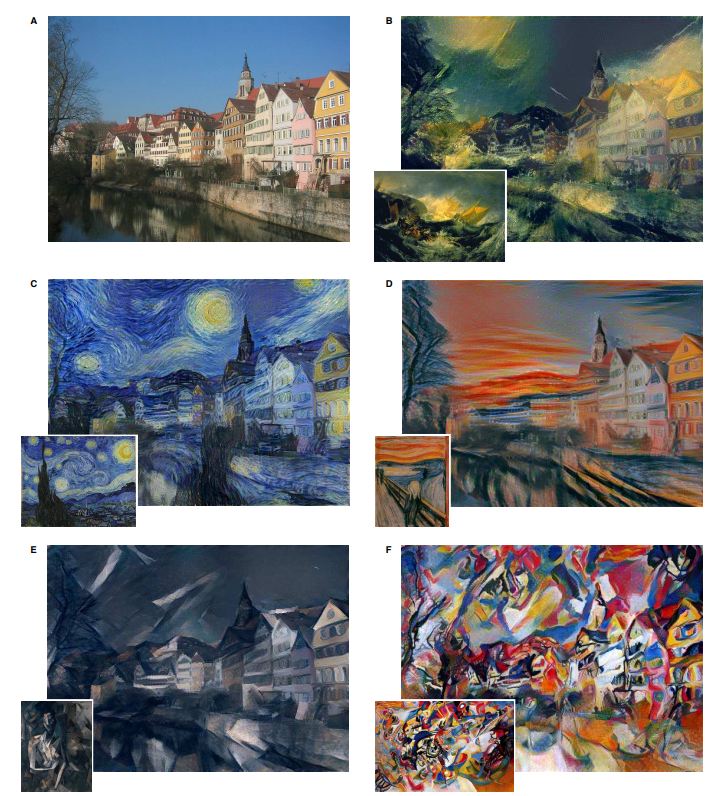
\includegraphics[width=130truemm]{resources/3_related_work/outputs_IST.pdf}
    \caption{
        Examples of images combining content and style, taken from
        \cite{Gatys_2016_CVPR}.
    }
    \label{output_IST}
\end{figure}
\clearpage

\section{Machines Painting Like Human Painters: DRL}
 Painting is a form of artistic expression that usually involving imaginative or 
creative skills, and it takes a lot of time and proper training to master the 
art.  Teaching a machine to paint is a challenging task, but researching it 
could lead to the development of tools that assist people in painting.

Huang \textit{et al}. \cite{Huang_2019_ICCV} trained a painting agent which 
imitates the painting process of humans. 
They employ a neural renderer in model-based deep reinforcement learning.
The agent is trained using model-based reinforcement learning, in which the 
agent learns to predict the outcomes of its actions and uses these predictions 
to plan its next actions, such as selecting a brush or color.
The agent is able to receive a larger reward as the visual quality of the 
paintings it create is better. The agent learns to make good painting choices by 
trying out various actions with the goal of maximizing the reward it receives.

It is demonstrated that their agent is able to learn to paint a variety of 
different styles and subjects, including handwritten digits, landscapes, 
portraits, and natural scene images. (Figure \ref{LearnToPaint})
\begin{figure}[h]
    \centering
    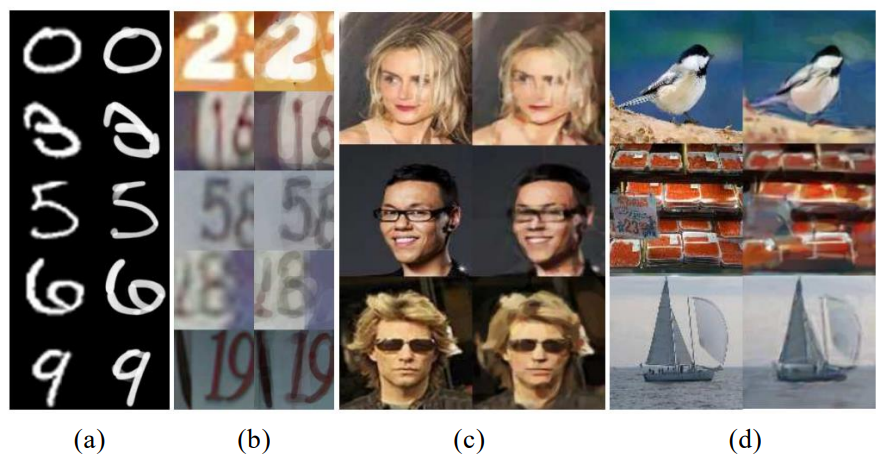
\includegraphics[width=120truemm]{resources/3_related_work/LearnToPaint.pdf}
    \caption{
        The painting results generated from the model introduced in the paper,
        taken from \cite{Huang_2019_ICCV}.
        (a) : MNIST dataset from \cite{deng2012mnist}. (b) SVHN dataset from \cite{netzer2011reading}.
        (c) : CelebA dataset from \cite{Liu_2015_ICCV}.
        (d) : ImageNet dataset from \cite{russakovsky2015imagenet}.
    }
    \label{LearnToPaint}
\end{figure}
\newline
As shown in Figure \ref{LearnToPaint}, the model-based deep reinforcement 
learning method generates attractive paintings, but there seems to be problems
such as long training time for the agent and the instability of the agent.

\section{Machines Painting Like Human Painters: FNNs}
 Liu \textit{et al}. \cite{liu2021paint} proposed Paint Transformer, a novel 
framework paintings from natural images by predicting parameters of multiple 
strokes without using reinforcement learning. 
Paint Transformer is a Transformer-based framework. This framework generates 
painting from natural images by using a feed-forward transformer to predict 
the multiple stroke parameters. 
Paint Transformer consists of two modules: the Stroke Predictor and the Stroke Renderer.  

In this work, strokes are represented by shape parameters ${x, y, h, w, \theta}$ 
and color parameters ${r, g, b}$.
\begin{figure}[h]
    \centering
    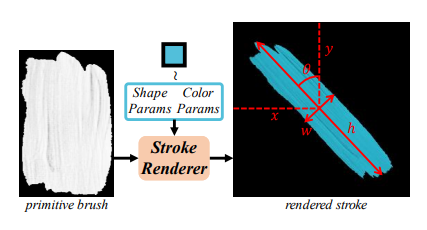
\includegraphics[width=110truemm]{resources/3_related_work/stroke-params.pdf}
    \caption{
        Parameter definition of a stroke,
        taken from \cite{liu2021paint}.
    }
    \label{strokeparams}
\end{figure}
\newline
The parameters are defined as shown in Figure \ref{strokeparams}, the center 
coordinates ($x$ and $y$), the height ($h$) and width ($w$) of the stroke, 
and the angle of rotation ($\theta$). Additionally, the RGB values of the 
stroke are represented by $r$, $g$, and $b$. Thus, the strokes generated are 
limited to monochromatic and linear.

Paint Transformer pipeline is shown in Figure \ref{PTpipeline}.
Stroke Predictor takes the target image It and the intermediate 
image $I_c$ as input, and generates a set of strokes $S_r$
(strictly speaking, it generates the parameters to determine the stroke set $S_r$).
The goal of training the Stroke Predictor is to make $S_r$ match a reference set
of strokes $S_f$. 
Stroke Renderer then takes each stroke in $S_r$ and generates a stroke image, 
which is combined with $I_c$ to create the final result image $I_r$.
This process can be expressed as follows:
\begin{equation}
    \label{painttransformer}
    I_r = PaintTransformer(I_c, I_t)
\end{equation}
\vspace{5mm}
\begin{figure}[t]
    \centering
    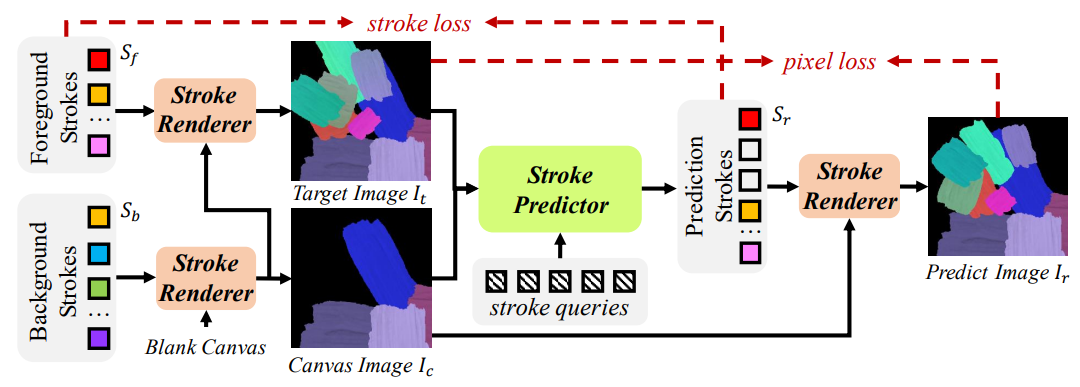
\includegraphics[width=140truemm]{resources/3_related_work/PTpipeline.pdf}
    \caption{
        A pipeline for Paint Transformer,
        taken from \cite{liu2021paint}.
    }
    \label{PTpipeline}
\end{figure}

\vspace{0.7cm}

\begin{figure}[h]
    \centering
    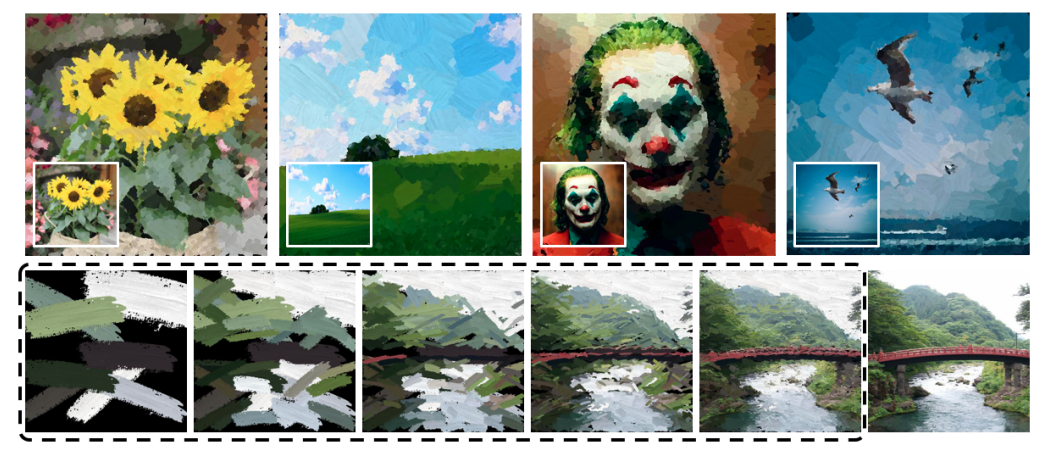
\includegraphics[width=135truemm]{resources/3_related_work/PTresult.pdf}
    \caption{
        The painting results generated from Paint Transformer,
        taken from \cite{liu2021paint}.
    }
    \label{PTresult}
\end{figure}
As shown in Figure \ref{PTresult}, this model produces highly quality paintings.
However, the strokes used are currently limited to monochromatic and linear forms.
To generate paintings with various touches, it should be explored more complex 
strokes with various shapes or color patterns.

